\documentclass[12pt, a4paper]{extarticle}


\usepackage{amsmath,amsthm,amssymb}
\usepackage{mathtext}	
\usepackage[T2A,T1]{fontenc}
\usepackage[utf8]{inputenc}
\usepackage{textcomp}
\usepackage[russian, english, ukrainian]{babel}
\usepackage{lmodern}
\usepackage{mathtools, amssymb}
\usepackage{bm}
\usepackage{hyperref}
\usepackage{longtable}
\usepackage{verbatim}
\usepackage[nottoc,numbib]{tocbibind}
\newcommand{\norm}[1]{\left\lVert#1\right\rVert}
\usepackage{multirow}

%\setlength{\parindent}{4em}
%\setlength{\parskip}{1em}
%\renewcommand{\baselinestretch}{1.5}

\newtheorem{algorithm}{Алгоритм}
\newtheorem{assumption}{Припущення}
\newtheorem{definition}{Визначення}
\newtheorem{theorem}{Теорема}




\begin{document}

\begin{titlepage}%
	\begin{center}
		{КИЇВСЬКИЙ НАЦІОНАЛЬНИЙ УНІВЕРСИТЕТ \\ІМЕНІ ТАРАСА ШЕВЧЕНКА}\par
		{ФAКУЛЬТЕТ КОМП'ЮТЕРНИХ НАУК ТА КІБЕРНЕТИКИ\\ КАФЕДРА ОБЧИСЛЮВАЛЬНОЇ МАТЕМАТИКИ}\par
		\begin{center}
			\begin{figure}[h]
				\center{
\includegraphics[width=0.3\linewidth]{figures/univ_logo.jpg}}
			\end{figure}
		\end{center}
		\vspace{3mm}
		\bf{\small{ВИПУСКНА КВАЛІФІКАЦІЙНА РОБОТА МАГІСТРА}}\par
	{\small{на тему:}}\par
			\vspace{10mm}
			{\LARGE{\bf{\scshape{Методи ідентифікації автора}}}}\par
			\vspace{5mm}
			{}\par %subtitle
	\end{center}
	\vfill
	\hfill
	\begin{flushright}
	\begin{minipage}[t]{85mm}
			\flushright
			Виконав\\
			студент 2-го курсу магістратури\\
			{Михайлюк Владислав Юрійович}\par
			\vspace{2ex}
			Науковий керівник:\\
			{доктор фізико-математичних наук}\\
			{Клюшин Дмитро Анатолійович}\par   
	\end{minipage}
	\end{flushright}
	\vspace{3mm}
	\begin{flushleft}
			%\begin{minipage}[t]{80mm}
			% TODO: коли роботу заслухано?
			%Роботу заслухано на засіданні кафедри обчислювальної математики та рекомендовано до захисту в ДЕК, протокол №8 від 24 травня 2018 р.\\
			%Завідувач кафедри обчислювальної математики проф. Ляшко С.І.
			%\end{minipage}
			\end{flushleft}
	\vfill
	\vspace{1mm}
	\begin{center}Київ --- 2020\end{center}
\end{titlepage}

\section{Зміст}
\tableofcontents
\newpage
\section{Вступ}
Література часто розглядається як предмет, який стосується лише читання та мислення. Але, як це відбувається майже у всіх областях інтелекту, воно перетинається з іншими. У своїй роботі "Принципи стильометрії" 1890 року польський філософ Вінсентій Лутославський використовував статистичні підходи для побудови хронології діалогів Платона. Кажуть, що стилометрія почалася, коли в 1851 році Август де Морган сказав про тексти біблійних авторів, що «один з авторів використовує довші слова». Стильометрія - лінгвістична дисципліна, яка застосовує статистичний аналіз до літератури шляхом оцінки авторського стилю за допомогою різних кількісних критеріїв. 

Розвиток копьютерів та їх можливостей для аналізу великох кільскоті данних створює можливості для дослудження більш складних статистичних методів. На тематику роботи з літературними творами та текстами існує багато
досліджень, які використовують різні методи та підходи до вирішення задачі. У роботах були розглянуті такі підходи, як глибинне навчання Liuyu Zhou\cite{NewsAuthorshipIdentificationwithDeepLearning},
Mike Kestemont\cite{OverviewoftheAuthorIdentificationTaskatPAN2018}, N. Smirnov\cite{Tableforestimatingthegoodnessoffitofempiricaldistributions}, класичні методи машинного навчання
Granichin\cite{WritingstyledeterminationusingtheKNNtextmodel}, Grieve\cite{QuantitativeauthorshipattributionAnevaluationoftechniques}, та статистичні методи Stamatatos\cite{Asurveyofmodernauthorshipattributionmethods}, Giacomo Inches\cite{FindingParticipantsinaChatAuthorshipAttributionforConversationalDocuments},
Shane Bergsma\cite{StylometricAnalysisofScientificArticles}, Борисов Л.А\cite{IdentificationAuthorByFrequencies}.

Питяння статистичного аналізу знаходиться у сфері інтересів як літературознавців, так і математиків. Цікавими є задачі кластеризації текстів за автором, жанром, форматов, епохою написання, чи емоційним забарвленням. Математичний інтерес полягаж в дослудженні алгоритмики процессу творчї роботи мозку. Також самостійну цінність мають і статистичні методи аналізу таких многомірних по своїм атрибутам об'єктам, як літературні тексти, написані професійними письменниками.

Найбільш популярною є задача ідентифікації авторства тексту. Для її вирішення досить часто використовуютья статичтичні методи, що грунтуються на припущенні, що письменник в своїх творах притримується певної поведінки письма, що формує певні інварінти, які підкреслють стилистичну характеристику творів автора. Такими інваріантами можуть бути кількісні ознаки долі голосних та приголосних у тексті, частота використання певних комбінацій слів, частота слів-маркерів. Практичне застосування це питання може знайти в пошуку плагіату, лінвістичних, історичних та кримінілістих дослідженнях.

У данній роботі проводиться порівняльний аналіз двох підходів для ідентифікації автора. Первший грунтується на порівнянні частот буквосполучень. Другий метод полягає у висуванні гіпотези про належність тексту до певного та доведення її з використанням p-статистики\cite{AnAssumptioninMachineLearning}. Також так як автори можуть писати в різних стилях, то використання одного еталону для автора може бути не ефективним. Тому розглядається також підхід з кластеризації текстів автора, і подальшому знаходженні еталону для кожного кластеру. Припускається, що такий елалон відповідає окремому стилю стилю автора. Кластеризація виконувалась ієрархічним методом кластерізації з "відстаню поділу авторів" $\hat{\rho}$, в якості параметру.\\
В алфавіті з 26 символами існує $26^3=17526$ різним $n$-грам довжиною 3, що накладає робичть обчислення відстані від автора до автора досить ресурсоємким, тому в данній роботі пропонується метод по знаходжненню найбільш ефективних $n$-грам для ідентифікації автора.


Головною метою данної роботи є порівняння методів з точки зору вікористания ресурсів, швидкості обчислень, складності реалізації та точності ідентифікації. Також в данній роботі достіджєються частоти n-грамм, як стилістичні характеристику тексту.

Так як автори можуть писати в різних стилях, то використання одного еталону для автора може бути не


\newpage
\section{Умовні позначення та терміни}
$A$ - кількість авторів\\
$m$ - кількість символів з алфавіту\\
Алфавіт надалі вважається фіксованим\\
$n$-грама - послідовність з $n$ символів алфавіту\\
$K_\alpha$ - кількість текстів автора $\alpha$\\
$N_{i,\alpha}$ - кількість букв в $i$-ому текті автора $\alpha$\\
$n$-ЩФР - щільність функції розподілу $n$-грамм тексту відповідного алфавіту\\
$f_{i,\alpha}(j)$ - $n$-ЩФР $i$-го текту автора $\alpha$, де аргумент $j$ відповідає деякому $n$-граму, та змінюється від $1$ до $m^n$\\ 
$f_{i,\alpha}^k(j)$ - $n$-ЩФР $k$-ої частини $i$-го текту автора $\alpha$, де аргумент $j$ відповідає деякому $n$-граму, та змінюється від $1$ до $a(n)=m^n$\\
$a(n)=m^n$ - кількість $n$-грам довжини $n$\\
$pstatistic(x,y)$ - міра однорідності двох вибірок, побудована 

\section{Методи}
\subsection{Щільність функції розподілу та її застосування для ідентифікації автора}
Нехай ми маємо бібліотеку, що містить тексти $A$ авторів. $K_\alpha$ - кількість наявних текстів автора. $N_{i,\alpha}$ - кількість букв в $i$-ому текті автора $\alpha$. Вважається, що довжина кожного з текстів достатня для проведення статистичного аналізу. Для кожного тексту знайдемо його представлення у вигляді частот $n$-грамм та позначимо $f_{i,\alpha}(j)$ відповідну $n$-ЩФР($n$-щільність функції розподілу) $i$-го текту автора $\alpha$, де аргумент $j$ відповідає деякому $n$-граму, та змінюється від $1$ до $a(n)=m^n$:
Для кожного автора визначимо його сереньозважену ЩФР\cite{Authoridentificationinshorttexts}:
\begin{equation} \label{eq:1}
F_{\alpha}(j) = \frac{1}{N_\alpha} \sum_{i=1}^{K_\alpha}f_{i,a}(j)N_{i,\alpha} 
\end{equation}
\begin{equation}\label{eq:2}
N_\alpha  = \sum_{i=1}^{K_\alpha}N_{i,a}
\end{equation}
Ці $n$-ЩФР далі будуть грати роль авторських еталонів.\\
В \ref{eq:1}, \ref{eq:2} знехтувано тим фактом, що кількість різних $n$-грам на $n-1$ менше кількості символів в тексті, так як $N_\alpha >> n$.\\
Введемо бібліотечну норму $\rho_{ik}$, як відстань між ЩФР текстів i та k:
\begin{equation}\label{eq:3}
\rho_{ik} = \Vert f_i - f_k\Vert = \sum_{j=1}^{a(n)}\mid f_i(j) - f_k(j)\mid
\end{equation}
Для кожного автора $\alpha$ побудуэмо щільність функцій розподілу $g_\alpha^+(\rho)$ відхилень $\rho_{i_\alpha,\alpha}$ "його текстів", а також розподіл $g_\alpha^-(\rho)$ відхилень текстів інщих авторів від його середньої $n$-ЩФР $F_\alpha$. Позначимо $G_\alpha^{\pm}(\rho)$ відповідні фуцнкії розподілу. Мінімальне значення $\rho$ при якому $G_\alpha^-(\rho)=1$, позначимо $\rho_\alpha^+$, а максимальне значення $\rho$ при якому $G_\alpha^(\rho)=0$, позначимо $\rho_\alpha^-$.\\
Смисл введених позначень в тому що, всі ЩФР текстів автора $\alpha$ знаходятся на відстані не більш ніж $\rho_\alpha^+$ від його середньої ЩФР $F_{\alpha}$, та аналогічно всі ЩФР текстів інших авторів знаходятся на відстані не менш $\rho_\alpha^-$. Величина $1-G_\alpha^+(\rho_\alpha^-)$ - ймовірність помилково ідентифікувати $\alpha$ як автора(помилка другого роду), а величина $G_\alpha^-(\rho_\alpha^+)$ - ймовірність помилково ідентифікувати текст автора $\alpha$, як текст написаний іншим автором(помилка першого роду).
Позначимо $G^+(\rho)$ - розподіл відхидень текстів від відповідних еталонів, та $G^-(\rho)$ - розподіл відхидень текстів від "чужих" еталонів:
\begin{equation}\label{eq:4}
G^+(\rho) = \frac{\sum_{\alpha=1}^{A} K_\alpha G_\alpha^+(\rho)}{\sum_{\alpha=1}^{A} K_\alpha}
\end{equation}
\begin{equation}\label{eq:5}
G^-(\rho) = \frac{\sum_{\alpha=1}^{A} K_\alpha G_\alpha^-(\rho)}{\sum_{\alpha=1}^{A} K_\alpha}
\end{equation}
 Назвемо вілстаню поділу авторів таке значення $\hat{\rho}$, для якої помилка ідентифікації автора тексту мінімальна:
\begin{equation}\label{eq:6}
\hat{\rho_\alpha} = argmin(1 - G_\alpha^+(\rho) + G_\alpha^-(\rho)) = argmax(G_\alpha^+(\rho) - G_\alpha^-(\rho))
\end{equation}
\begin{equation}\label{eq:7}
\hat{\rho} = argmin(1 - G^+(\rho) + G^-(\rho)) = argmax(G^+(\rho) - G^-(\rho))
\end{equation}
Величина $\hat{\rho}$ може слугувати верхнім рівнем кластерізації текстів.

Нехай тепер ми маэмо текст "0", автора якого треба ідентифікувати. Тоді автором текста вважається той автор $\alpha$, для якого норма $\rho_\alpha = \Vert f_0-F_\alpha \Vert$ різноці між ЩФР $f_0(j)$ текста "0" та середньої авторської ЩФР $F_\alpha(j)$ мінімальна:
\begin{equation}\label{eq:8}
\rho_\alpha = \Vert f_0-F_\alpha \Vert, \;\;\;\; \alpha^0 = \underset{\alpha}{argmin} \rho_\alpha^0
\end{equation}
Правило \ref{eq:8} застосовується тільки в тому випадку, якщо $\min_\alpha \rho_\alpha^0 \leq \hat{\rho}$. Якщо $\min_\alpha \rho_\alpha^0 > \hat{\rho}$ - приймається рішення, що в данній бібліотеці немає відповідного автора.

\subsection{Метод з використанням з p-статистики}
\subsubsection{P-статистика}
P-значення(P-value),P-статистика  - вірогідність заданої статистичної моделі для якої, при умові що нульова гіпотеза є істиною, статистичні суми будуть однакові або матимуть більш екстремальні значення ніж для фактично отриманих результатів.\\
Нехай маємо дві вибірки $x=(x_1,x_2,...,x_n)$ $y=(y_1, y_2,...,y_m)$ з генеральних сукупностей $X$ та $Y$ відповідно. Для вибірки z відомо, що вона належить $X$ чи $Y$ - задача полягає у ідентифікації до якох саме сукупності належить z. Покладемо гіпотезу $H$ про однорідність двох вибірок з генеральних сукупностей з функціями розподілу $F_x(u)$ та $F_y(u)$ відповідно, $x=(x_1, x_2, ..., x_n)\in X$тТа $y=(y_1, y_2, ..., y_m)\in Y$ - тестові вибірки у яких виконуєтсья $x_1 \leq ... \leq x_n$ та $y_1 \leq ... \leq y_m$. Нехай гіпотеза $H$ полягає в $F_x(u)=F_y(u)$, тоді відповідно до $A(n)$ припущення Хілла:

\begin{equation}\label{eq:9}
p(y_k \in (x_i, x_j)) = \frac{j-i}{n+1}, i<j
\end{equation}
Використовуючи вибірку $y=(y_1, y_2,...,y_m)$, ми можемо частоту $h_{ij}$ випадкової події $y_k \in (x_i, x_j))$ та розрахувати довірчий інтервал $I_{ij}$ для ймовірності $p(y_k \in (x_i, x_j))$ з заданим рівнем значущості $\beta$.
Позначимо $L$ кількість інтервалів для яких виконується $frac{j-i}{n+1} \in I_{ij}$. Тоді, визначимо міру одноріності вибірок $x$ та $y$, як пропорцію інтервалів для яких вірно $frac{j-i}{n+1} \in I_{ij}$ серед усіх інтервалів:
\begin{equation}\label{eq:10}
h_{xy} = \frac{2L}{n*(n-1)}
\end{equation}
Так як, $h_{xy}$ - частота випадкової події $frac{j-i}{n+1} \in I_{ij}$ з  ймовірністю $1-\beta$, ми можемо побудувати довірчий інтервал $I_{xy}$ для події $frac{j-i}{n+1} \in I_{ij}$ з рівнем значущості $\beta$. Якщо $1-\beta \in I$ тоді гіпотеза $H$ підтверджена, інакше відхилена. Показник $h_{xy}$ є мірою однорідності вибірок $x$ та $y$. Змінивши $x$ та $y$ місцями та знайшовши частоту $h_{yx}$ та довірчий інтервал $I_{yx}$ ми можемо побудувати ще один тест для перевірки гіпотези $H$. Так як міра $h_{xy}$ не симетрична, ми можемо побудувати симетричну міру однорідності:
\begin{equation}\label{eq:11}
h = pstatistic(x,y) = \frac{1}{2}(h_{xy}+h_{yx})
\end{equation}

\subsubsection{Адаптація P-статистики для ідентифікації автора тексту. Вариант 1}
Нехай маємо бібліотеку з попереднього методу з $K_\alpha$ творами автора $\alpha$, $\alpha$ змінюється від 1 до $A$. Кожен текст в бібліотеці розібьємо на $K$ частин, та для кожноъ частини знайдемо $f_{i,\alpha}^k(j)$ - $n$-ЩФР $k$-ої частини тексту. Позначимо $g_{i,\alpha(j)}(j)$ множину множину частот $j$-ого $n$-граму $j$-ого тексту автора $\alpha$:
\begin{equation}\label{eq:12}
g_{i,\alpha}(j) = \{f_{i,\alpha}^1(j), f_{i,\alpha}^2(j), ..., f_{i,\alpha}^K(j)\}
\end{equation}
Тоді введемо відстань між текстами $a$ та $b$, як частина $n$-грам, для яких відхиляється гіпотеза про однорідність вибірок $g_a(j) = \{f_a^1(j), f_a^2(j), ..., f_a^K(j)\}$ та $g_b(j) = \{f_b^1(j), f_b^2(j), ..., f_b^K(j)\}$:
\begin{equation}\label{eq:14}
\Vert f_a^{(.)}-f_b^{(.)}\Vert = 1-\frac{\sum_{j=1}^{a(n)}pstatistic(g_a(j),g_b(j)}{a(n)}
\end{equation}
%\begin{equation}\label{eq:13}
%\Vert f_a^{(.)}-f_b^{(.)}\Vert = 1-\frac{\sum_{j=1}^{a(n)}H_0(g_a(j),g_b(j)}{a(n)}
%\end{equation}
%$H_0(x,y)=1$, якщо гіпотезу про однорідність вибірок $x$ та $y$ підтверджено, інакше - $H_0(x,y)=0$.\\
%Розглянемо алгоритм побудови елатону для автора $\alpha$. Для кожного $n$-граму треба знайти множину частот %розміром $K$, яка представляє розподіл $n$-грам цього автора. побудуємо множину частот $j$-ого $n$-граму $M=\%{f_{i,\alpha}^k(j)\}_{i=1..K_\alpha, k=1..K}$, відсортуємо множину $M$ за зростанням, та з відсортованого %кортежу виберемо $K$ елементів з кроком $K_\alpha$ починаючи з $\lfloor K/2 \rfloor$. Отриману множину частот %будемо використовувати як набір частот $j$-ого $n$-граму для еталону автора $\alpha$.

%\subsubsection{Адаптація P-статистики для ідентифікації автора тексту}
%Ще один вариант - використовувати в якості відстані між авторами $a$ та $b$:
%\begin{equation}\label{eq:14}
%\Vert f_a^{(.)}-f_b^{(.)}\Vert = 1-\frac{\sum_{j=1}^{a(n)}pstatistic(g_a(j),g_b(j)}{a(n)}
%\end{equation}


\newpage
\section{Обчислювальні експерименти}
\subsection{Інструменти розробки}

Бібліотека з текстами була завантажена з сайту \texttt{https://www.gutenberg.org/}, яка містить більш 60000 книг. Программа для завантаження бібліотеки написана на мові програмування \texttt{NodeJS v.12.13.1}.\\
Алгоритм для тестів розроблений на мові програмування \texttt{C++ 17}.Для підвищення швидкості обчислень використовувалися паралельні потоки.\\
Для візуалізації даних було використано \texttt{jupyter python}.\\
Тестування проводилось на комп'ютері із наступними специфікаціями:
\begin{itemize}
	\item \textbf{ОС:} \texttt{64bit Windows 10 Pro}
	\item \textbf{Центральний процесор:} \texttt{Processor	Intel(R) Core(TM) i7-7700HQ CPU @ 2.80GHz, 2801 Mhz, 4 Core(s), 8 Logical Processor(s)}
	\item \textbf{Оперативна пам'ять:} \texttt{32.0 GB}
\end{itemize}

\subsection{Вхідні дані}
Тестування проводилося на сукпності текстів 16 авторів: George Manville Fenn, Sir Walter Scott, R.M. Ballantyne, U.S. Copyright Office, Robert Louis Stevenson, Jules Verne, W.H.G. Kingston, George Sand, 
Anthony Trollope, Charles Dickens, G. A. Henty, Mór Jókai, Fergus Hume, Alexandre Dumas, E. Phillips Oppenheim, William Le Queux. Кожен автор має щонаймеш 50 книг довжиною 200000 символів в бібліотеці. Тести проводилися з використанням 5000, 10000, 20000, 50000, 100000, 200000 перших символів текстів. Тексти кожного автора було розділено на тренувальну та тестову вибірки по 25 текстів в кожній.\\
Так як обчислення відстанней для триграм ресурсоємке, були відібрані найбільш "впливові" триграми, тобто такі які найбільше відрізняють одоного автора від іншого. У якості міри "впливовості" була обрана наступна статистика:

\begin{equation}\label{eq:15}
v(j) = \frac{\sum_{\alpha=1}^{A}D(f_{\cdot,\alpha}(j))}{D(f_{\cdot.\cdot}(j))}
\end{equation}
\begin{equation}\label{eq:16}
D(f_{\cdot.\cdot}(j)) = \frac{\sum_{\alpha=1}^A \sum_{i=1}^{K_\alpha} (f_{i,\alpha}(j) - M(f_{\cdot.\cdot}(j)))^2}{\sum_{\alpha=1}^A K_\alpha}
\end{equation}
\begin{equation}\label{eq:17}
M(f_{\cdot.\cdot}(j)) = \frac{\sum_{\alpha=1}^A \sum_{i=1}^{K_\alpha} f_{i,\alpha}(j)}{\sum_{\alpha=1}^A K_\alpha}
\end{equation}
\begin{equation}\label{eq:18}
D(f_{\cdot.\alpha}(j)) = \frac{\sum_{i=1}^{K_\alpha} (f_{i,\alpha}(j) - M(f_{\cdot.\cdot}(j)))^2}{K_\alpha}
\end{equation}
\begin{equation}\label{eq:19}
M(f_{\cdot.\alpha}(j)) = \frac{\sum_{i=1}^{K_\alpha} f_{i,\alpha}(j)}{K_\alpha}
\end{equation}

$D(\cdot)$ - це дисперсія, а $M(\cdot)$ - матсподівання. Отримуємо, що $v(j)$ - показує яку частину загальної варіації частот $j$-ого $n$-граму складає варіація цих частот локальна по авторам. Якщо $v(j)$ близьке до 0 - це означає, що при зміні автора тексту ця частота змінюється значно більше ніж при зміні текст на текст того ж автора. Серед усіх $17526$ триграм було обрано $1802$ з мірою "впливовості" менше 0.6.

\begin{comment}
Далі, наведено триграми з відповідними мірами:\\
gup : 0.0679196, cco : 0.110757, oki : 0.136786, dnt : 0.141677, hno : 0.143705, rnd : 0.144935, kdo : 0.15108, kis : 0.151748, abo : 0.168971, bac : 0.175842, ash : 0.179805, wan : 0.179887, oer : 0.188652, won : 0.189046, dli : 0.191501, cri : 0.195873, may : 0.196517, ylo : 0.19856, get : 0.204317, gfa : 0.204775, khe : 0.208556, oka : 0.210412, ike : 0.217017, ced : 0.218456, uni : 0.223655, okh : 0.224504, nga : 0.22499, sib : 0.227588, nki : 0.230815, lik : 0.231286, tme : 0.235084, ook : 0.237076, lya : 0.23767, lld : 0.239534, tgo : 0.240002, ons : 0.242398, cci : 0.243383, ecr : 0.245022, cka : 0.247162, few : 0.248481, fel : 0.249381, sai : 0.254367, oee : 0.256303, ehy : 0.256508, way : 0.258001, awa : 0.258035, ivd : 0.259013, eis : 0.260023, ull : 0.260478, eco : 0.261364, wni : 0.261566, sre : 0.266072, epl : 0.266207, ddo : 0.266597, dly : 0.267403, twr : 0.268264, ugh : 0.269092, oug : 0.26989, inm : 0.27017, eor : 0.270384, ksa : 0.273256, ink : 0.273415, goa : 0.273993, xci : 0.275386, pre : 0.276949, fco : 0.277857, tnd : 0.277891, ybu : 0.278282, ket : 0.280459, ats : 0.281792, wwa : 0.28268, goi : 0.283131, upt : 0.283501, hin : 0.284019, hak : 0.286057, hyh : 0.286659, bou : 0.286953, shw : 0.287717, gru : 0.289772, ied : 0.290213, mil : 0.290743, epr : 0.291366, ckl : 0.291946, hho : 0.293931, thm : 0.29405, boy : 0.295665, aid : 0.296273, big : 0.297329, ldl : 0.297642, hom : 0.298857, kes : 0.299557, izo : 0.300468, knd : 0.301143, ebo : 0.301246, rep : 0.301563, rwr : 0.301858, ewm : 0.303121, owl : 0.304707, nkw : 0.304766, iva : 0.30481, cid : 0.306634, pfo : 0.307128, veg : 0.308772, ign : 0.309536, oin : 0.310164, nwo : 0.310546, upw : 0.31375, oko : 0.316087, eer : 0.317816, lov : 0.319517, fmi : 0.320115, oot : 0.32092, hyw : 0.32092, occ : 0.321618, dcl : 0.322814, dow : 0.324348, got : 0.324353, ped : 0.324521, wid : 0.325142, tel : 0.325396, ddr : 0.326667, tra : 0.327466, rhy : 0.327846, aft : 0.328079, afe : 0.328096, vew : 0.329054, gda : 0.329069, keh : 0.329628, hdw : 0.330332, meh : 0.330627, kwe : 0.332779, abl : 0.332887, dnd : 0.333379, beg : 0.333444, hbu : 0.334255, bew : 0.334521, gsh : 0.334634, rly : 0.335086, ndl : 0.335719, ing : 0.335761, loo : 0.335761, stn : 0.335831, ifw : 0.337212, kca : 0.338022, jac : 0.338981, tly : 0.339128, mak : 0.339132, wor : 0.33975, oyh : 0.339785, mom : 0.34025, pin : 0.3411, kwa : 0.342081, rwa : 0.342121, tst : 0.342374, ovd : 0.342824, dri : 0.343314, oze : 0.343329, rew : 0.343651, osi : 0.34397, tno : 0.344118, gve : 0.344234, thn : 0.344721, wto : 0.345046, lln : 0.345221, atc : 0.345376, bso : 0.345938, uri : 0.347891, wix : 0.347995, dgo : 0.348315, spo : 0.348361, pno : 0.34844, pto : 0.348725, sia : 0.349058, opp : 0.349541, bho : 0.350421, dba : 0.350453, rki : 0.350534, gso : 0.350631, ile : 0.351528, raf : 0.351877, adl : 0.352383, ttl : 0.352551, fal : 0.35295, mwo : 0.353101, mon : 0.353152, wly : 0.35332, pro : 0.353499, cie : 0.353533, tup : 0.353967, pyi : 0.355621, thy : 0.356151, kto : 0.356345, dne : 0.356427, upe : 0.356564, osw : 0.356615, pyd : 0.356694, rwo : 0.356913, rul : 0.357275, gri : 0.357699, gab : 0.357781, kas : 0.358468, pby : 0.358764, fas : 0.359079, con : 0.359194, ply : 0.359477, ysh : 0.359652, rou : 0.35967, cks : 0.35976, xtm : 0.359914, dez : 0.360011, dhy : 0.360296, led : 0.360366, ake : 0.360676, yan : 0.361016, app : 0.361287, vdh : 0.361712, dkn : 0.36224, lyh : 0.362428, jus : 0.362481, its : 0.362621, ohe : 0.362849, lnd : 0.363342, tli : 0.363667, kli : 0.363807, dke : 0.363877, oww : 0.364025, osh : 0.364569, lds : 0.365201, ack : 0.365281, wkw : 0.365386, utt : 0.367352, ifi : 0.367623, hyy : 0.367792, oyw : 0.368623, owh : 0.368796, ghi : 0.3688, ief : 0.369175, shd : 0.369841, fei : 0.369987, eow : 0.370283, low : 0.370783, kor : 0.371105, avo : 0.371423, usa : 0.371596, myl : 0.371758, llh : 0.371949, wmo : 0.37263, kfu : 0.372704, sho : 0.373344, llw : 0.373347, isa : 0.373348, wst : 0.374213, stm : 0.374433, ibl : 0.374496, uwe : 0.374532, eep : 0.374549, hal : 0.374562, avy : 0.375689, kst : 0.376022, shy : 0.37621, rvd : 0.376298, old : 0.376345, ble : 0.37666, kle : 0.377837, cir : 0.377877, apr : 0.378138, gsa : 0.378328, ndh : 0.378564, wsa : 0.378571, rue : 0.378681, itw : 0.379078, ngs : 0.379337, gon : 0.379556, llm : 0.380926, fyo : 0.381253, gcr : 0.381381, dma : 0.381468, gho : 0.38161, nyt : 0.381727, lri : 0.381854, rhe : 0.382178, wlo : 0.382435, row : 0.382459, her : 0.3826, tcr : 0.382795, doa : 0.383328, ndm : 0.383417, obs : 0.383964, nbu : 0.383983, omp : 0.384026, edo : 0.384434, cte : 0.384635, tsh : 0.384986, idt : 0.385068, lke : 0.385222, rig : 0.385268, snd : 0.385564, gnd : 0.385779, ssi : 0.386603, ads : 0.386819, gba : 0.387135, evo : 0.387239, fmy : 0.388634, gaz : 0.388719, sse : 0.388943, own : 0.389215, gfo : 0.389261, esa : 0.389434, ksi : 0.389504, wri : 0.389721, dbo : 0.38984, ntk : 0.390793, ega : 0.391041, gai : 0.391102, gst : 0\\
\end{comment}


\subsection{Метод з використанням щільністі функції розподілу}
У таблицях \ref{tab:1}, \ref{tab:2}, \ref{tab:3} міститься інфирмація про середні відстані текстів до єталонів кожного автора для монограмів, біграмів, триграмів відповідно. А на рисунках \ref{fig:1}, \ref{fig:2}, \ref{fig:3} зображені щільністі розподілів відстаней до еталонів $n$-грам. З отриманих таблиц бачимо, що Jules Verne, Charles Dickens та Alexandre Dumas - мають досить великі середні відстані до власного еталону, це  пояснюється тим, що ці автори пишуть в досить різних стилях.
\begin{center}
\begin{table}
\begin{tabular}{|p{11em}|p{5em}|p{5em}|p{5em}|p{5em}|}
\hline
\multirow{2}{4em}{Автор} & \multicolumn{2}{|p{10em}|}{Середня відстань власних текстів до еталону} & \multicolumn{2}{|p{10em}|}{Середня відстань чужих текстів до еталону} \\
\cline{2-5}
& Навчальна вибірка & Тестова вибірка & Навчальна вибірка & Тестова вибірка\\
\hline
George Manville Fenn & 0.0338465 & 0.0340254 & 0.148186 & 0.160377\\
Sir Walter Scott & 0.0284826 & 0.0663677 & 0.134049 & 0.147205\\
R.M. Ballantyne & 0.0256525 & 0.0259007 & 0.132092 & 0.146816\\
U.S. Copyright Office & 0.0474249 & 0.0434929 & 0.230926 & 0.241641\\
Robert Louis Stevenson & 0.0660438 & 0.0500744 & 0.13504 & 0.150064\\
Jules Verne & 0.194515 & 0.232865 & 0.214297 & 0.223655\\
W.H.G. Kingston & 0.0310675 & 0.0344322 & 0.140399 & 0.153805\\
George Sand & 0.0345426 & 0.0521552 & 0.345482 & 0.354845\\
Anthony Trollope & 0.0312901 & 0.0393127 & 0.144474 & 0.157774\\
Charles Dickens & 0.137723 & 0.201273 & 0.147524 & 0.156707\\
G. A. Henty & 0.0299935 & 0.0315441 & 0.141307 & 0.155087\\
Mór Jókai & 0.23157 & 0.221696 & 0.266655 & 0.265208\\
Fergus Hume & 0.0346095 & 0.0355302 & 0.132482 & 0.146382\\
Alexandre Dumas & 0.10102 & 0.152488 & 0.283127 & 0.291188\\
E. Phillips Oppenheim & 0.0273646 & 0.0319321 & 0.136483 & 0.150508\\
William Le Queux & 0.0312424 & 0.0289607 & 0.131785 & 0.145958\\
\hline
\end{tabular}
\caption{Порівняння відстаней до еталонів. Монограми.}
\label{tab:1}
\end{table}
\end{center}
\begin{figure}
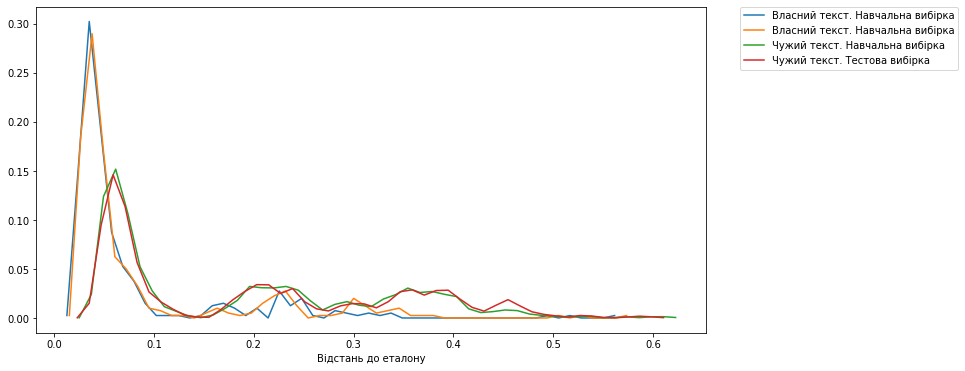
\includegraphics[width=\linewidth]{figures/1.png}
\centering
\caption{Щільність розподілу відстаней. Монограми.}
\label{fig:1}
\end{figure}

\begin{center}
\begin{table}
\begin{tabular}{|p{11em}|p{5em}|p{5em}|p{5em}|p{5em}|}
\hline
\multirow{2}{4em}{Автор} & \multicolumn{2}{|p{10em}|}{Середня відстань власних текстів до еталону} & \multicolumn{2}{|p{10em}|}{Середня відстань чужих текстів до еталону} \\
\cline{2-5}
& Навчальна вибірка & Тестова вибірка & Навчальна вибірка & Тестова вибірка\\
\hline
George Manville Fenn & 0.0994828 & 0.100713 & 0.337656 & 0.364495\\
Sir Walter Scott & 0.0857056 & 0.160734 & 0.312519 & 0.337815\\
R.M. Ballantyne & 0.0842319 & 0.0831463 & 0.303563 & 0.333081\\
U.S. Copyright Office & 0.142319 & 0.131085 & 0.518372 & 0.536536\\
Robert Louis Stevenson & 0.153465 & 0.126039 & 0.305945 & 0.336367\\
Jules Verne & 0.434099 & 0.507919 & 0.467984 & 0.481571\\
W.H.G. Kingston & 0.0986361 & 0.101119 & 0.319829 & 0.347821\\
George Sand & 0.0953532 & 0.131873 & 0.720437 & 0.736496\\
Anthony Trollope & 0.0978328 & 0.120733 & 0.335552 & 0.363841\\
Charles Dickens & 0.289434 & 0.424478 & 0.322943 & 0.339882\\
G. A. Henty & 0.0958608 & 0.0976739 & 0.32082 & 0.349905\\
Mór Jókai & 0.473379 & 0.450451 & 0.564311 & 0.563759\\
Fergus Hume & 0.103849 & 0.110262 & 0.308154 & 0.336897\\
Alexandre Dumas & 0.228394 & 0.34131 & 0.612664 & 0.625097\\
E. Phillips Oppenheim & 0.0855664 & 0.0948044 & 0.316374 & 0.344707\\
William Le Queux & 0.0926607 & 0.0948494 & 0.306627 & 0.334875\\
\hline
\end{tabular}
\caption{Порівняння відстаней до еталонів. Біграми.}
\label{tab:2}
\end{table}
\end{center}
\begin{figure}
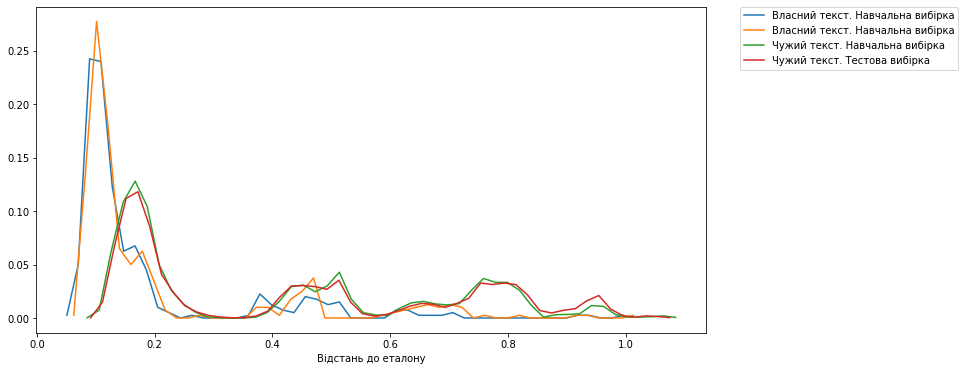
\includegraphics[width=\linewidth]{figures/2.png}
\centering
\caption{Щільність розподілу відстаней. Монограми.}
\label{fig:2}
\end{figure}

\begin{center}
\begin{table}
\begin{tabular}{|p{11em}|p{5em}|p{5em}|p{5em}|p{5em}|}
\hline
\multirow{2}{4em}{Автор} & \multicolumn{2}{|p{10em}|}{Середня відстань власних текстів до еталону} & \multicolumn{2}{|p{10em}|}{Середня відстань чужих текстів до еталону} \\
\cline{2-5}
& Навчальна вибірка & Тестова вибірка & Навчальна вибірка & Тестова вибірка\\
\hline
George Manville Fenn & 0.180418 & 0.18861 & 0.596302 & 0.623662\\
Sir Walter Scott & 0.171463 & 0.283575 & 0.524401 & 0.549622\\
R.M. Ballantyne & 0.172195 & 0.169814 & 0.51445 & 0.545968\\
U.S. Copyright Office & 0.283822 & 0.276685 & 0.815953 & 0.833536\\
Robert Louis Stevenson & 0.259684 & 0.228195 & 0.511306 & 0.545252\\
Jules Verne & 0.655446 & 0.770669 & 0.789989 & 0.801207\\
W.H.G. Kingston & 0.194357 & 0.204415 & 0.539513 & 0.568905\\
George Sand & 0.162869 & 0.224804 & 1.15696 & 1.16934\\
Anthony Trollope & 0.185929 & 0.224242 & 0.572796 & 0.603712\\
Charles Dickens & 0.466389 & 0.668956 & 0.530902 & 0.546114\\
G. A. Henty & 0.189261 & 0.19251 & 0.539592 & 0.571259\\
Mór Jókai & 0.632626 & 0.749113 & 0.671995 & 0.671159\\
Fergus Hume & 0.192996 & 0.206572 & 0.530133 & 0.561459\\
Alexandre Dumas & 0.368591 & 0.561702 & 1.02425 & 1.02995\\
E. Phillips Oppenheim & 0.170172 & 0.19042 & 0.546378 & 0.576854\\
William Le Queux & 0.194836 & 0.198912 & 0.520049 & 0.550307\\
\hline
\end{tabular}
\caption{Порівняння відстаней до еталонів. Біграми.}
\label{tab:3}
\end{table}
\end{center}
\begin{figure}
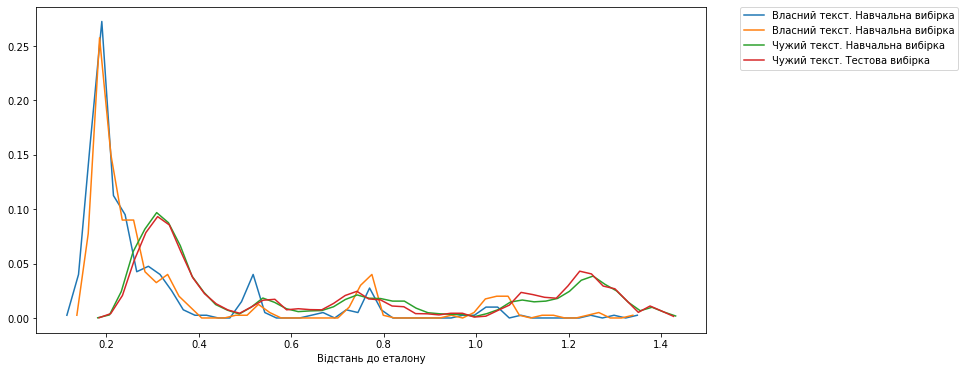
\includegraphics[width=\linewidth]{figures/3.png}
\centering
\caption{Щільність розподілу відстаней. Триграми.}
\label{fig:3}
\end{figure}
На рисунку \ref{fig:4} зображена точність ідентифікації авторів для різної довжини текстів. Можна помітити, що для точність ідентифікації текстів за допомогою біграм та триграм на тестовій вибірці місцями перевищує точність ідентифікації на навчальній вибірці. Це пояснюється тим, що до тестової вибірки потрапили більш вузькі за своїм стилем тексти.
0.7725 0.785 0.7375 0.76 0.695 0.6875

\begin{center}
\begin{table}
\begin{tabular}{|p{5em}|p{10em}|p{10em}|}
\hline
& Навчальна вибірка & Тестова вибірка\\
\hline
монограми & 0.695 & 0.6875\\
біграми & 0.7375 & 0.765\\
триграми & 0.7725 & 0.785\\
\hline
\end{tabular}
\caption{Точність для тексту в 200000 символів. Метод з використанням щільністі функції розподілу}
\label{tab:4}
\end{table}
\end{center}
\begin{figure}
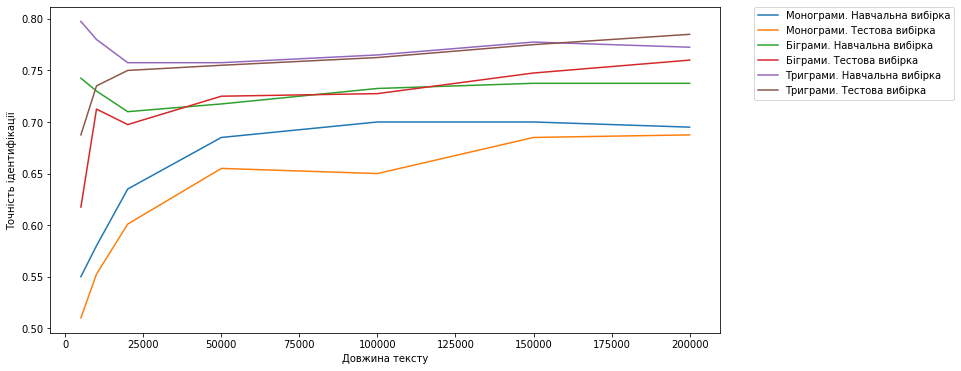
\includegraphics[width=\linewidth]{figures/4.png}
\centering
\caption{Точність ідентифікації для різної довжини текстів.}
\label{fig:4}
На рисунку \ref{fig:5} зображена точність ідентифікації авторів для різної довжини n-грам. 
\end{figure}
\begin{figure}
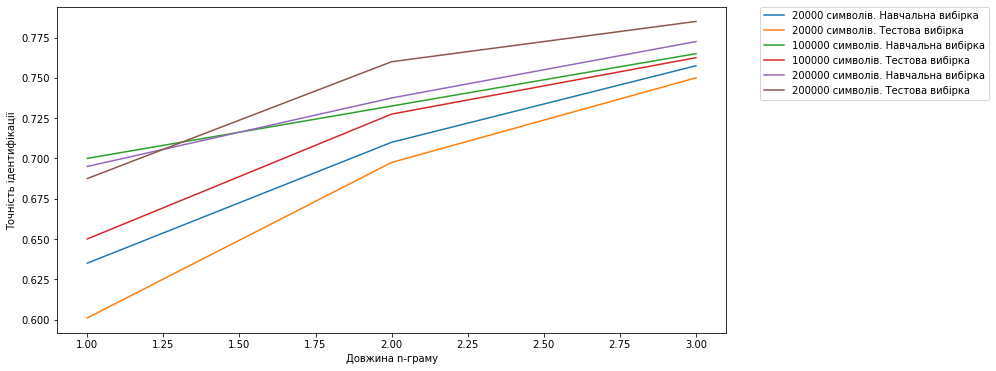
\includegraphics[width=\linewidth]{figures/5.png}
\centering
\caption{Точність ідентифікації для різної довжини n-грам}
\label{fig:5}
\end{figure}
Можна зробити такі висновки:
- Починаючи з довжини тексту в 20000 сиволів зміна похибки точністі ідентифікації для біграм та трирам  незначна(1-2\%), а починаючи з 50000 сиволів зміна похибки для монограм також незначна.
\subsection{Метод з використанням p-статистики}
На рисунку \ref{fig:6} зображена залежність точності ідентифікації автора залежно від довжини тексту для K=20. Спостерігаємо, що загалом зі збільшенням довжини текстів, збільшується точність ідентифікації. Також між тестовими та навчальними вибірками є розрив в 5-10\% точності.

\begin{figure}
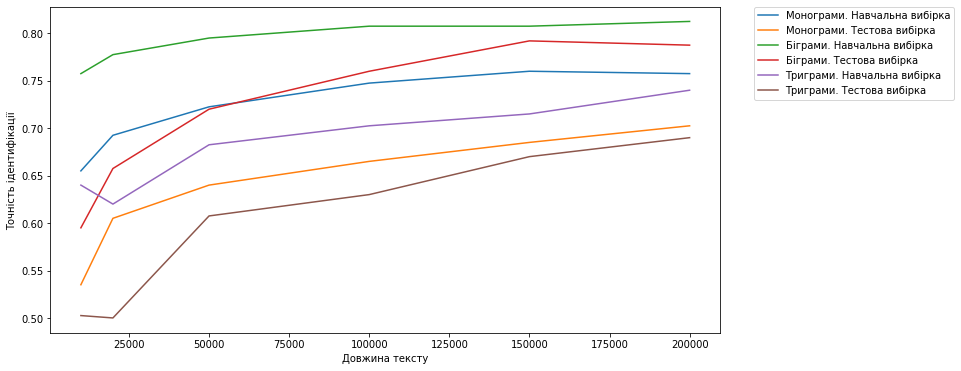
\includegraphics[width=\linewidth]{figures/6.png}
\centering
\caption{Точність ідентифікації для різної довжини текстів. K=20}
\label{fig:6}
На рисунку \ref{fig:6} зображена залежність точності ідентифікації залежно від кількості частин на які розбивався текст. При збільшенні кількості частин тексту точність ідентифікації точність ідентифікації триграмами різко зменшується, що означає що, довжина тексту недостатня для отримання високох точності. При збільшенні кількості частин тексту точність ідентифікації для біграм та монограм зменшується незначно. Для Біграм найбільш ефективним є розбиття K=7, для монограм K=15, для триграм K=3. На рисунку \ref{fig:8} зображено залежність точності ідентицікації для відповідних розбиттів. Бачимо що для триграм навіть при розбитті на 3 частини 200000 символів в тексті недостатньо для досягнення околу статистичної границі.
\end{figure}
\begin{figure}
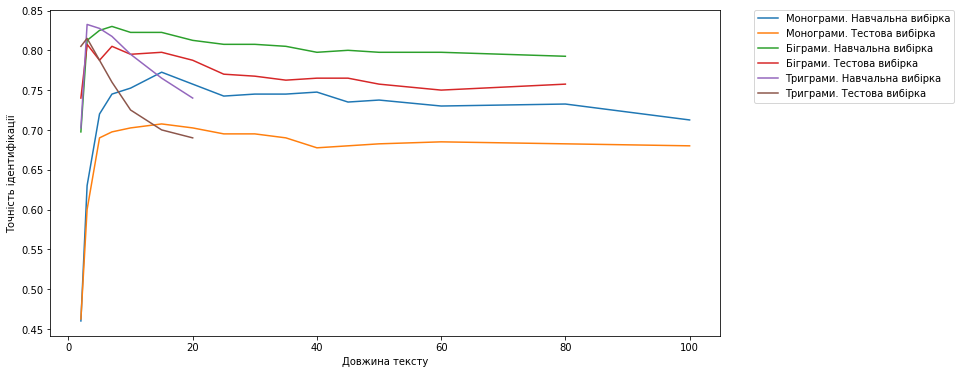
\includegraphics[width=\linewidth]{figures/7.png}
\centering
\caption{Точність ідентифікації різних розбиттів. Добвжина текстів 200000}
\label{fig:7}
\end{figure}
\begin{figure}
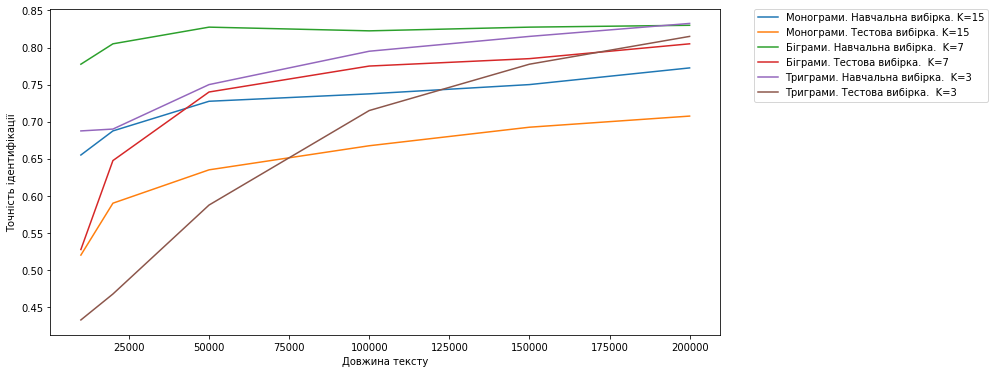
\includegraphics[width=\linewidth]{figures/8.png}
\centering
\caption{Точність ідентифікації для різної довжини текстів. K=15 для монограм, K=7 для біграм, K=3 для триграм}
\label{fig:8}
\end{figure}
\begin{center}
\begin{table}
\begin{tabular}{|p{5em}|p{10em}|p{10em}|}
\hline
& Навчальна вибірка & Тестова вибірка\\
\hline
монограми & 0.7725 & 0.7075\\
біграми & 0.83 & 0.8055\\
триграми & 0.8325 & 0.815\\
\hline
\end{tabular}
\caption{Точність для тексту в 200000 символів. P-статистика.}
\label{tab:5}
\end{table}
\end{center}
\subsection{Кластерізація}
Так як автори можуть писати в різних стилях, кластерізація текстів автора з подальшим знаходженням еталону для кожного автора може бути досить ефективною. В якості методу кластерізації було обрано ієрархічний метод кластерізації, так як в метод можна передати максимальну відстань між кластерами. У якості параметру використовулася міра поділу авторів(Таблиці \ref{tab:6}, \ref{tab:7}, \ref{tab:8} для монограм, біграм та триграм відповідно). У таблицях \ref{tab:9},\ref{tab:10}, \ref{tab:11} знаходяться кількість кластерів по  авторам для моногрма, біграм та триграм відповідно.

\begin{center}
\begin{table}
\begin{tabular}{|p{11em}|p{10em}|p{10em}|}
\hline
Автор & $\hat{\rho_\alpha}$ для метод з використанням щільністі функції розподілу & $\hat{\rho_\alpha}$ для метод з використанням p-статистики\\
\hline
George Manville Fenn & 0.0463045 & 0.187912\\
Sir Walter Scott & 0.0375501 & 0.158608 \\
R.M. Ballantyne & 0.0318236 & 0.143223\\
U.S. Copyright Office & 0.0657424 & 0.176374\\
Robert Louis Stevenson & 0.0543053 & 0.209341\\
Jules Verne & 0.178568 & 0.365568\\
W.H.G. Kingston & 0.0397744 & 0.157326\\
George Sand & 0.0549845 & 0.249267\\
Anthony Trollope & 0.0426615 & 0.172711\\
Charles Dickens & 0.0823775 & 0.224908\\
G. A. Henty & 0.04078 & 0.177473\\
Mór Jókai & 0.247522 & 0.335897\\
Fergus Hume & 0.0374213 & 0.170879\\
Alexandre Dumas & 0.0929762 & 0.259524\\
E. Phillips Oppenheim & 0.0411207 & 0.17619\\
William Le Queux & 0.0387453 & 0.172344\\
\hline
\end{tabular}
\caption{$\hat{\rho_\alpha}$. Монограми}
\label{tab:6}
\end{table}
\end{center}
\begin{center}
\begin{table}
\begin{tabular}{|p{11em}|p{10em}|p{10em}|}
\hline
Автор & $\hat{\rho_\alpha}$ для метод з використанням щільністі функції розподілу & $\hat{\rho_\alpha}$ для метод з використанням p-статистики\\
\hline
George Manville Fenn & 6 & 4\\
Sir Walter Scott & 4 & 6\\
R.M. Ballantyne & 5 & 3\\
U.S. Copyright Office & 1 & 1\\
Robert Louis Stevenson & 5 & 8\\
Jules Verne & 4 & 4\\
W.H.G. Kingston & 4 & 7\\
George Sand & 1 & 1\\
Anthony Trollope & 5 & 3\\
Charles Dickens & 3 & 5\\
G. A. Henty & 2 & 1\\
Mór Jókai & 2 & 2\\
Fergus Hume & 5 & 9\\
Alexandre Dumas & 2 & 2\\
E. Phillips Oppenheim & 1 & 1\\
William Le Queux & 5 & 6\\
\hline
\end{tabular}
\caption{Кількість кластерів. Триграми}
\label{tab:9}
\end{table}
\end{center}




\begin{center}
\begin{table}
\begin{tabular}{|p{11em}|p{10em}|p{10em}|}
\hline
Автор & $\hat{\rho_\alpha}$ для метод з використанням щільністі функції розподілу & $\hat{\rho_\alpha}$ для метод з використанням p-статистики\\
\hline
George Manville Fenn & 0.0463045 & 0.187912\\
Sir Walter Scott & 0.0375501 & 0.158608 \\
R.M. Ballantyne & 0.0318236 & 0.143223\\
U.S. Copyright Office & 0.0657424 & 0.176374\\
Robert Louis Stevenson & 0.0543053 & 0.209341\\
Jules Verne & 0.178568 & 0.365568\\
W.H.G. Kingston & 0.0397744 & 0.157326\\
George Sand & 0.0549845 & 0.249267\\
Anthony Trollope & 0.0426615 & 0.172711\\
Charles Dickens & 0.0823775 & 0.224908\\
G. A. Henty & 0.04078 & 0.177473\\
Mór Jókai & 0.247522 & 0.335897\\
Fergus Hume & 0.0374213 & 0.170879\\
Alexandre Dumas & 0.0929762 & 0.259524\\
E. Phillips Oppenheim & 0.0411207 & 0.17619\\
William Le Queux & 0.0387453 & 0.172344\\
\hline
\end{tabular}
\caption{$\hat{\rho_\alpha}$. Біграми}
\label{tab:7}
\end{table}
\end{center}

\begin{center}
\begin{table}
\begin{tabular}{|p{11em}|p{10em}|p{10em}|}
\hline
Автор & $\hat{\rho_\alpha}$ для метод з використанням щільністі функції розподілу & $\hat{\rho_\alpha}$ для метод з використанням p-статистики\\
\hline
George Manville Fenn & 1 & 1\\
Sir Walter Scott & 2 & 3\\
R.M. Ballantyne & 3 & 3\\
U.S. Copyright Office & 1 & 10\\
Robert Louis Stevenson & 6 & 7\\
Jules Verne & 4 & 2\\
W.H.G. Kingston & 6 & 4\\
George Sand & 1 & 1\\
Anthony Trollope & 1 & 3\\
Charles Dickens & 3 & 4\\
G. A. Henty & 1 & 1\\
Mór Jókai & 2 & 1\\
Fergus Hume & 13& 1\\
Alexandre Dumas & 2 & 2\\
E. Phillips Oppenheim & 1 & 1\\
William Le Queux & 7 & 7\\
\hline
\end{tabular}
\caption{Кількість кластерів. Триграми}
\label{tab:10}
\end{table}
\end{center}

\begin{center}
\begin{table}
\begin{tabular}{|p{11em}|p{10em}|p{10em}|}
\hline
Автор & $\hat{\rho_\alpha}$ для метод з використанням щільністі функції розподілу & $\hat{\rho_\alpha}$ для метод з використанням p-статистики\\
\hline
George Manville Fenn & 0.236771 & 0.269608\\
Sir Walter Scott & 0.24953 & 0.266926\\
R.M. Ballantyne & 0.200519 & 0.258232\\
U.S. Copyright Office & 0.363961 & 0.275157\\
Robert Louis Stevenson & 0.237309 & 0.264058\\
Jules Verne & 0.724427 & 0.349427\\
W.H.G. Kingston & 0.209656 & 0.268868\\
George Sand & 0.221383 & 0.338605\\
Anthony Trollope & 0.246643 & 0.27525\\
Charles Dickens & 0.312767 & 0.285331\\
G. A. Henty & 0.225755 & 0.274972\\
Mór Jókai & 0.508067 & 0.321032\\
Fergus Hume & 0.231127 & 0.264058\\
Alexandre Dumas & 0.333833 & 0.348594\\
E. Phillips Oppenheim & 0.218364 &0.270533\\
William Le Queux & 0.22903 & 0.26859\\
\hline
\end{tabular}
\caption{$\hat{\rho_\alpha}$. Триграми}
\label{tab:8}
\end{table}
\end{center}
\begin{center}
\begin{table}
\begin{tabular}{|p{11em}|p{10em}|p{10em}|}
\hline
Автор & $\hat{\rho_\alpha}$ для метод з використанням щільністі функції розподілу & $\hat{\rho_\alpha}$ для метод з використанням p-статистики\\
\hline
George Manville Fenn & 1 & 1\\
Sir Walter Scott & 2 & 21\\
R.M. Ballantyne & 3 & 4\\
U.S. Copyright Office & 1 & 9\\
Robert Louis Stevenson & 6 & 7\\
Jules Verne & 3 & 4\\
W.H.G. Kingston & 6 & 5\\
George Sand & 1 & 3\\
Anthony Trollope & 1 & 1\\
Charles Dickens & 3 & 5\\
G. A. Henty & 6 & 1\\
Mór Jókai & 2 & 7\\
Fergus Hume & 2 & 12\\
Alexandre Dumas & 2 & 2\\
E. Phillips Oppenheim & 1 & 1\\
William Le Queux & 8 & 5\\
\hline
\end{tabular}
\caption{Кількість кластерів. Триграми}
\label{tab:11}
\end{table}
\end{center}

\begin{center}
\begin{table}
\begin{tabular}{|p{5em}|p{10em}|p{10em}|}
\hline
& Навчальна вибірка & Тестова вибірка\\
\hline
монограми & 0.9125 & 0.75\\
біграми & 0.98 & 0.8925\\
триграми & 0.99 & 0.9175\\
\hline
\end{tabular}
\caption{Точність методу з використанням щільністі функції розподілу з кластерізацією}
\label{tab:12}
\end{table}
\end{center}

\begin{center}
\begin{table}
\begin{tabular}{|p{5em}|p{10em}|p{10em}|}
\hline
& Навчальна вибірка & Тестова вибірка\\
\hline
монограми & 0.97 & 0.8125\\
біграми & 0.91 & 0.8525\\
триграми & 0.9875 & 0.805\\
\hline
\end{tabular}
\caption{Метод з використанням p-статистики. K=15 для монограм, K=7 для біграм, K=3 для триграм}
\label{tab:13}
\end{table}
\end{center}

\section{Аналіз результатів}
\subsection{Час виконання}
Метод з використанням щільністі функції розподілу виявився значино швидшим за метод з використанням p-статистики, за рахунок того, що для p-статистики треба розрахувати $\frac{K(K-1)}{2}$ довірчих інтервалів для кожного $n$-граму, у порівнянні з суммою різниць частот $n$-граму.
\subsection{Точність ідентифікації}
Для монограм, біграм та триграм метод з використанням p-статистики дає кращі результати в точності на $3-4\%$(для текстів довжиною більше 50000). Однак для невеликих за розміром текстів p-статистика дає гірші результати, ніж метод з використанням щільністі функції розподілу.\\

З використанням кластерізації точність на тестовій виборці зросла приблизно на $5\%$ для монограм, та на приблизно на $10\%$ для біграм та триграм у випадку методу з використанням щільністі функції розподілу, та найкращу точність в $91.75\%$ було отримано для триграм. У випадку методу з використанням p-статистики точність для монограм та триграм зросла приблизно на $5\%$, а для триграм майже не змінилася, та найкращу точність в $85.25\%$ було отримано для біграм.\\
З отриманих результатів можна зробити висновки:
- у випадку кластерізації метод з використанням щільністі функції розподілу дає кращі результати. Тому саме розподіл частот деякого $n$-граму не дає більше інформації о стилю, в якому пише автор, ніж середнє цього розподілу.
- В данному контексті, виходячи з попеднього пункту, P-статистику, можна вважати деякою емпіричною версією аналогією довірчого інтервалу, так як без кластерізації p-статистика давала кращі результати, а з кластерізацією - гірші.
- розподіл $n$-грамів дійсно змінюється зі зміною стилю, однак, для отримання більших точностей, необхідно шукати інші маркери

\section{Висновки}
У результаті дослідження було реалізовано 2 методи ідентифікації невідомого автора твору, який належить до бібліотеки відомих авторів, також реалізовано метод кластрізації текстів та проведено тестування методів з та без кластерізацією. Також було запропоновано метод критерій для відбору $n$-грам, які б найкраще слугували маркером для ідентифікації автора. Для тестування використовувалися 800 текстів 16 авторів. В результаті було виявлено, що методу, що використовує щільність функції розподілу підходить для ідентифікації авторів творів як великих текстів(50000+ симолів) так и малих(10000+ символів). А метод, що використовує p-статистику підходить тільки для використання на великих за обсягов творах. З кластерізацією текстів були отримані значно кращі результати на тестовій вибірці для обох методів.

\bibliographystyle{plain}
\bibliography{diploma} 

\end{document}
